

\tikzset{every picture/.style={line width=0.75pt}} %set default line width to 0.75pt        

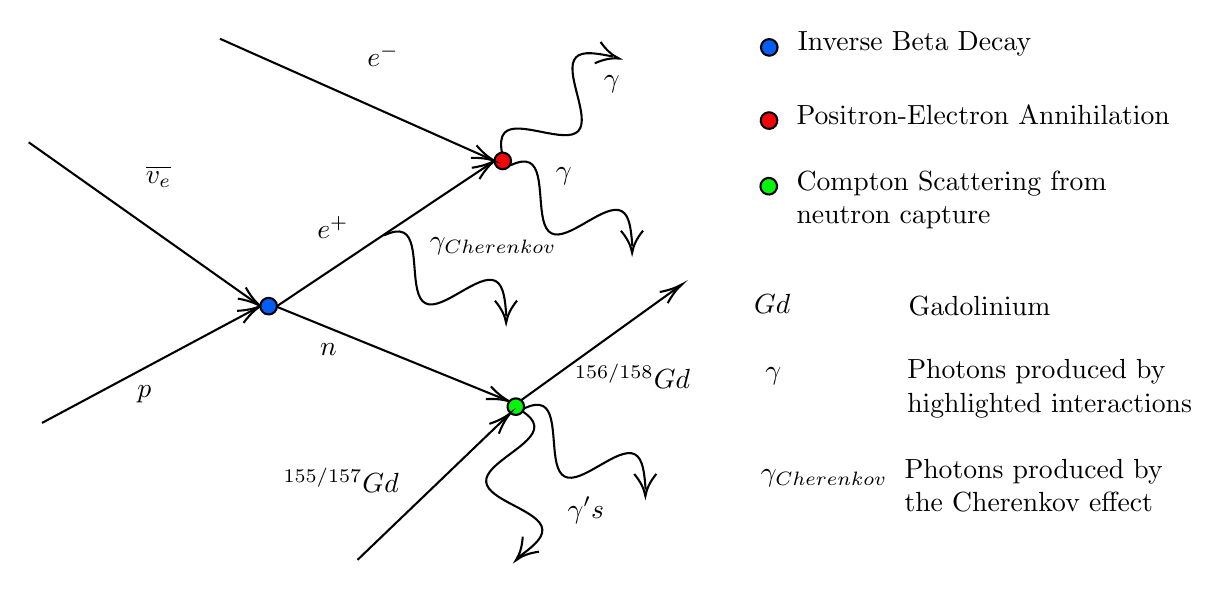
\begin{tikzpicture}[x=0.75pt,y=0.75pt,yscale=-1,xscale=1]
%uncomment if require: \path (0,526); %set diagram left start at 0, and has height of 526

%Straight Lines [id:da6653054220109853] 
\draw    (35.4,187.4) -- (145.37,265.18) ;
\draw [shift={(147,266.33)}, rotate = 215.27] [color={rgb, 255:red, 0; green, 0; blue, 0 }  ][line width=0.75]    (10.93,-3.29) .. controls (6.95,-1.4) and (3.31,-0.3) .. (0,0) .. controls (3.31,0.3) and (6.95,1.4) .. (10.93,3.29)   ;
%Straight Lines [id:da8296039138645427] 
\draw    (41.8,322.6) -- (145.24,267.28) ;
\draw [shift={(147,266.33)}, rotate = 511.86] [color={rgb, 255:red, 0; green, 0; blue, 0 }  ][line width=0.75]    (10.93,-3.29) .. controls (6.95,-1.4) and (3.31,-0.3) .. (0,0) .. controls (3.31,0.3) and (6.95,1.4) .. (10.93,3.29)   ;
%Straight Lines [id:da09351342912264893] 
\draw    (155,266.67) -- (265.15,311.45) ;
\draw [shift={(267,312.2)}, rotate = 202.12] [color={rgb, 255:red, 0; green, 0; blue, 0 }  ][line width=0.75]    (10.93,-3.29) .. controls (6.95,-1.4) and (3.31,-0.3) .. (0,0) .. controls (3.31,0.3) and (6.95,1.4) .. (10.93,3.29)   ;
%Straight Lines [id:da23693990731168424] 
\draw    (155,266.33) -- (258.14,197.44) ;
\draw [shift={(259.8,196.33)}, rotate = 506.26] [color={rgb, 255:red, 0; green, 0; blue, 0 }  ][line width=0.75]    (10.93,-3.29) .. controls (6.95,-1.4) and (3.31,-0.3) .. (0,0) .. controls (3.31,0.3) and (6.95,1.4) .. (10.93,3.29)   ;
%Shape: Circle [id:dp5776429452576024] 
\draw  [fill={rgb, 255:red, 5; green, 94; blue, 244 }  ,fill opacity=1 ] (147,266.33) .. controls (147,264.12) and (148.79,262.33) .. (151,262.33) .. controls (153.21,262.33) and (155,264.12) .. (155,266.33) .. controls (155,268.54) and (153.21,270.33) .. (151,270.33) .. controls (148.79,270.33) and (147,268.54) .. (147,266.33) -- cycle ;
%Shape: Circle [id:dp7394219068166704] 
\draw  [fill={rgb, 255:red, 244; green, 5; blue, 5 }  ,fill opacity=1 ] (263.85,192.38) .. controls (266.05,192.4) and (267.82,194.22) .. (267.8,196.42) .. controls (267.77,198.63) and (265.96,200.4) .. (263.75,200.38) .. controls (261.55,200.35) and (259.77,198.54) .. (259.8,196.33) .. controls (259.83,194.12) and (261.64,192.35) .. (263.85,192.38) -- cycle ;
%Shape: Circle [id:dp34500649776325787] 
\draw  [fill={rgb, 255:red, 5; green, 244; blue, 11 }  ,fill opacity=1 ] (267,312.2) .. controls (268.41,310.5) and (270.93,310.26) .. (272.63,311.67) .. controls (274.33,313.08) and (274.57,315.61) .. (273.16,317.31) .. controls (271.75,319.01) and (269.23,319.24) .. (267.53,317.83) .. controls (265.83,316.42) and (265.59,313.9) .. (267,312.2) -- cycle ;
%Straight Lines [id:da6481294917609935] 
\draw    (127.53,137.5) -- (241.3,188.11) -- (257.97,195.52) ;
\draw [shift={(259.8,196.33)}, rotate = 203.98] [color={rgb, 255:red, 0; green, 0; blue, 0 }  ][line width=0.75]    (10.93,-3.29) .. controls (6.95,-1.4) and (3.31,-0.3) .. (0,0) .. controls (3.31,0.3) and (6.95,1.4) .. (10.93,3.29)   ;
%Straight Lines [id:da9680665411342746] 
\draw    (193.8,388.6) -- (266.08,319.22) ;
\draw [shift={(267.53,317.83)}, rotate = 496.17] [color={rgb, 255:red, 0; green, 0; blue, 0 }  ][line width=0.75]    (10.93,-3.29) .. controls (6.95,-1.4) and (3.31,-0.3) .. (0,0) .. controls (3.31,0.3) and (6.95,1.4) .. (10.93,3.29)   ;
%Straight Lines [id:da726424591273459] 
\draw    (272.63,311.67) -- (348.58,256.97) ;
\draw [shift={(350.2,255.8)}, rotate = 504.23] [color={rgb, 255:red, 0; green, 0; blue, 0 }  ][line width=0.75]    (10.93,-3.29) .. controls (6.95,-1.4) and (3.31,-0.3) .. (0,0) .. controls (3.31,0.3) and (6.95,1.4) .. (10.93,3.29)   ;
%Shape: Wave [id:dp6924354718089606] 
\draw  [color={rgb, 255:red, 0; green, 0; blue, 0 }  ,draw opacity=1 ] (271.27,387.38) .. controls (277.4,382.82) and (283.22,378.45) .. (282.87,373.94) .. controls (282.53,369.43) and (276.09,366.02) .. (269.34,362.45) .. controls (262.59,358.89) and (256.16,355.48) .. (255.81,350.96) .. controls (255.46,346.45) and (261.29,342.09) .. (267.41,337.53) .. controls (273.53,332.97) and (279.36,328.6) .. (279.01,324.09) .. controls (278.8,321.35) and (276.34,319.01) .. (272.92,316.8) ;
\draw   (281.22,384.65) .. controls (276.64,385.24) and (272.92,386.63) .. (270.07,388.83) .. controls (272.05,385.83) and (273.16,382.01) .. (273.41,377.4) ;
%Shape: Wave [id:dp07230520631582671] 
\draw  [color={rgb, 255:red, 0; green, 0; blue, 0 }  ,draw opacity=1 ] (332.64,354.72) .. controls (332.04,347.11) and (331.45,339.85) .. (327.45,337.74) .. controls (323.45,335.64) and (317.13,339.26) .. (310.52,343.08) .. controls (303.9,346.89) and (297.59,350.52) .. (293.58,348.41) .. controls (289.58,346.3) and (288.99,339.05) .. (288.39,331.43) .. controls (287.79,323.82) and (287.21,316.56) .. (283.2,314.46) .. controls (280.77,313.18) and (277.48,314.01) .. (273.79,315.73) ;
\draw   (337.79,347.17) .. controls (334.85,350.74) and (333.09,354.3) .. (332.52,357.86) .. controls (331.91,354.3) and (330.11,350.76) .. (327.13,347.23) ;

%Shape: Wave [id:dp22661760017094512] 
\draw  [color={rgb, 255:red, 0; green, 0; blue, 0 }  ,draw opacity=1 ] (265.54,271.22) .. controls (264.94,263.61) and (264.35,256.35) .. (260.35,254.24) .. controls (256.35,252.14) and (250.03,255.76) .. (243.42,259.58) .. controls (236.8,263.39) and (230.49,267.02) .. (226.48,264.91) .. controls (222.48,262.8) and (221.89,255.55) .. (221.29,247.93) .. controls (220.69,240.32) and (220.11,233.06) .. (216.1,230.96) .. controls (213.67,229.68) and (210.38,230.51) .. (206.69,232.23) ;
\draw   (270.69,263.67) .. controls (267.75,267.24) and (265.99,270.8) .. (265.42,274.36) .. controls (264.81,270.8) and (263.01,267.26) .. (260.03,263.73) ;




%Shape: Wave [id:dp24682356020386254] 
\draw  [color={rgb, 255:red, 0; green, 0; blue, 0 }  ,draw opacity=1 ] (326.24,237.52) .. controls (325.64,229.91) and (325.05,222.65) .. (321.05,220.54) .. controls (317.05,218.44) and (310.73,222.06) .. (304.12,225.88) .. controls (297.5,229.69) and (291.19,233.32) .. (287.18,231.21) .. controls (283.18,229.1) and (282.59,221.85) .. (281.99,214.23) .. controls (281.39,206.62) and (280.81,199.36) .. (276.8,197.26) .. controls (274.37,195.98) and (271.08,196.81) .. (267.39,198.53) ;
\draw   (331.39,229.97) .. controls (328.45,233.54) and (326.69,237.1) .. (326.12,240.66) .. controls (325.51,237.1) and (323.71,233.56) .. (320.73,230.03) ;


%Shape: Wave [id:dp5371122247315074] 
\draw  [color={rgb, 255:red, 0; green, 0; blue, 0 }  ,draw opacity=1 ] (316.8,146.06) .. controls (309.31,144.58) and (302.17,143.18) .. (299.06,146.47) .. controls (295.95,149.76) and (297.73,156.81) .. (299.62,164.21) .. controls (301.5,171.61) and (303.29,178.67) .. (300.18,181.96) .. controls (297.07,185.24) and (289.92,183.85) .. (282.43,182.37) .. controls (274.94,180.89) and (267.79,179.5) .. (264.68,182.78) .. controls (262.79,184.78) and (262.71,188.17) .. (263.36,192.19) ;
\draw   (310.93,139.06) .. controls (313.57,142.85) and (316.52,145.51) .. (319.79,147.02) .. controls (316.21,146.65) and (312.32,147.43) .. (308.11,149.33) ;

%Shape: Circle [id:dp3323147223186588] 
\draw  [fill={rgb, 255:red, 5; green, 94; blue, 244 }  ,fill opacity=1 ] (388.2,141.67) .. controls (388.2,139.46) and (389.99,137.67) .. (392.2,137.67) .. controls (394.41,137.67) and (396.2,139.46) .. (396.2,141.67) .. controls (396.2,143.88) and (394.41,145.67) .. (392.2,145.67) .. controls (389.99,145.67) and (388.2,143.88) .. (388.2,141.67) -- cycle ;
%Shape: Circle [id:dp40944776553384055] 
\draw  [fill={rgb, 255:red, 244; green, 5; blue, 5 }  ,fill opacity=1 ] (389.01,174.37) .. controls (390.42,172.67) and (392.94,172.43) .. (394.64,173.84) .. controls (396.34,175.25) and (396.58,177.77) .. (395.17,179.47) .. controls (393.76,181.17) and (391.23,181.41) .. (389.53,180) .. controls (387.83,178.59) and (387.6,176.07) .. (389.01,174.37) -- cycle ;
%Shape: Circle [id:dp020015830997712647] 
\draw  [fill={rgb, 255:red, 5; green, 244; blue, 11 }  ,fill opacity=1 ] (388.87,206) .. controls (390.28,204.3) and (392.8,204.06) .. (394.5,205.47) .. controls (396.2,206.88) and (396.44,209.41) .. (395.03,211.11) .. controls (393.62,212.81) and (391.09,213.04) .. (389.39,211.63) .. controls (387.69,210.22) and (387.46,207.7) .. (388.87,206) -- cycle ;



% Text Node
\draw (90.33,197.3) node [anchor=north west][inner sep=0.75pt]    {$\overline{v_{e}}$};
% Text Node
\draw (86.23,303.13) node [anchor=north west][inner sep=0.75pt]    {$p$};
% Text Node
\draw (172.93,221.7) node [anchor=north west][inner sep=0.75pt]    {$e^{+}$};
% Text Node
\draw (174.3,282.77) node [anchor=north west][inner sep=0.75pt]    {$n$};
% Text Node
\draw (197.03,138.7) node [anchor=north west][inner sep=0.75pt]    {$e^{-}$};
% Text Node
\draw (156.7,342.87) node [anchor=north west][inner sep=0.75pt]    {$^{155/157} Gd$};
% Text Node
\draw (297.1,292.53) node [anchor=north west][inner sep=0.75pt]    {$^{156/158} Gd$};
% Text Node
\draw (293.53,356.9) node [anchor=north west][inner sep=0.75pt]    {$\gamma 's$};
% Text Node
\draw (227.23,231.6) node [anchor=north west][inner sep=0.75pt]    {$\gamma _{Cherenkov}$};
% Text Node
%\draw (17.03,218) node [anchor=north west][inner sep=0.75pt]    {$\gamma _{Cherenkov}$};
% Text Node
\draw (287.93,197.9) node [anchor=north west][inner sep=0.75pt]    {$\gamma $};
% Text Node
\draw (311.03,153.9) node [anchor=north west][inner sep=0.75pt]    {$\gamma $};
% Text Node
\draw (404.53,132.67) node [anchor=north west][inner sep=0.75pt]   [align=left] {Inverse Beta Decay};
% Text Node
\draw (403.87,168) node [anchor=north west][inner sep=0.75pt]   [align=left] {Positron-Electron Annihilation};
% Text Node
\draw (403.87,200) node [anchor=north west][inner sep=0.75pt]   [align=left] {Compton Scattering from \\neutron capture};
% Text Node
\draw (383.37,259.07) node [anchor=north west][inner sep=0.75pt]    {$Gd$};
% Text Node
\draw (388.87,294.57) node [anchor=north west][inner sep=0.75pt]    {$\gamma $};
% Text Node
\draw (386.7,343.73) node [anchor=north west][inner sep=0.75pt]    {$\gamma _{Cherenkov}$};
% Text Node
\draw (457.87,260) node [anchor=north west][inner sep=0.75pt]   [align=left] {Gadolinium};
% Text Node
\draw (457.2,290.67) node [anchor=north west][inner sep=0.75pt]   [align=left] {Photons produced by\\highlighted interactions};
% Text Node
\draw (455.87,338.67) node [anchor=north west][inner sep=0.75pt]   [align=left] {Photons produced by\\the Cherenkov effect};


\end{tikzpicture}
